\documentclass[conference]{IEEEtran}
\usepackage{cite}
\usepackage{amsmath,amssymb,amsfonts}
\usepackage{algorithmic}
\usepackage{graphicx}
\usepackage{textcomp}
\usepackage{xcolor}
\def\BibTeX{{\rm B\kern-.05em{\sc i\kern-.025em b}\kern-.08em
    T\kern-.1667em\lower.7ex\hbox{E}\kern-.125emX}}
\begin{document}
\selectlanguage{dutch}

\title{Digitale kunstcollecties ontdekken door middel van Link-Traversal–based Query Processing}

\author{\IEEEauthorblockN{Martijn Bogaert}
\IEEEauthorblockA{
\textit{Universiteit Gent}\\
Gent, België \\
martijn.bogaert@ugent.be}}

\maketitle

\begin{abstract}
Deze masterproef onderzoekt het verkennen van digitale kunstcollecties via Link-Traversal-based Querying, met de focus op de \textit{Collectie van de Gentenaar}. Het Comunica-platform speelt een sleutelrol bij het benutten van waardevolle data in RDF-formaat, hoewel sommige links uitdagingen met RDF-compatibiliteit opleveren. Twee webapplicatie-ideeën worden voorgesteld om zowel gebruikers zonder technische achtergrond als professionals te helpen bij het verkennen van de CoGent-collectie. Het einddoel is om ontdekte data te koppelen aan IIIF Manifests voor visualisatie en zo de toegankelijkheid van kunstcollecties te vergroten.
\end{abstract}

\begin{IEEEkeywords}
Linked Data, Link Traversal, LTQP, CoGent, IIIF
\end{IEEEkeywords}

\section*{Inleiding}
Digitale kunstcollecties belichamen menselijke creativiteit en culturele ontwikkeling. Door technologische vooruitgang zijn deze verzamelingen gedigitaliseerd, waardoor ze wereldwijd toegankelijk zijn en diepgaand kunnen worden verkend. Toch brengt het navigeren en bevragen van deze gegevens uitdagingen met zich mee, vooral voor niet-technische professionals en kunstliefhebbers. Deze beperking belemmert hun vermogen om inzichten te verwerven en volledig op te gaan in de wereld van digitale kunst.

De culturele data van de Collectie van de Gentenaar (CoGent) worden gepubliceerd volgens de principes van Linked Data, waardoor ze stevig verankerd zijn in het semantische web. Maar om het volledige potentieel van deze uitgebreide gegevens te benutten, is Link-Traversal–based Query Processing (LTQP) vereist. LTQP stelt gebruikers namelijk in staat om buiten de grenzen van de dataset te treden, waardoor lagen van kennis en verbindingen kunnen worden blootgelegd die anders verborgen zouden blijven.

Het onderzoek ontleedt het \textit{ontdekken} van de CoGent-gegevens in drie fundamentele onderdelen: het opstellen van queries, het uitvoeren van queries met behulp van linktraversal - de van het onderzoek - en het verwerken van queryresultaten, met name de visualisatie en opslag ervan. Deze opgedeelde aanpak legt de basis voor een diepgaandere verkenning van de CoGent-data en mogelijks digitale kunstcollecties in het algemeen.

\section{Gerelateerd werk}
TODO

\subsection{Collectie van de Gentenaar}
TODO

\subsection{International Image Interoperability Framework}
TODO

\subsection{Link-Traversal-based Query Processing}
TODO

\section{CoGent data en link traversal}
TODO

\subsection{CoGent databronnen}
TODO

\subsection{Comunica link traversal engine configuratie}
TODO

\subsection{Te volgen links}
TODO

\section{Tools voor de constructie van query's}
TODO

\subsection{Queryconstructie door middel van predicaatsequenties}
TODO

\subsection{Gebruikersgerichte applicaties}
TODO

\section{Queryresultaten verwerken}
TODO

\subsection{Queryresultaten visualiseren}
TODO

\subsection{Queryresultaten opslaan}
TODO

\section*{Dankwoord}
TODO

% \bibliographystyle{IEEEtran}
% \bibliography{references}

\end{document}


% \begin{table}[htbp]
% \caption{Table Type Styles}
% \begin{center}
% \begin{tabular}{|c|c|c|c|}
% \hline
% \textbf{Table}&\multicolumn{3}{|c|}{\textbf{Table Column Head}} \\
% \cline{2-4} 
% \textbf{Head} & \textbf{\textit{Table column subhead}}& \textbf{\textit{Subhead}}& \textbf{\textit{Subhead}} \\
% \hline
% copy& More table copy$^{\mathrm{a}}$& &  \\
% \hline
% \multicolumn{4}{l}{$^{\mathrm{a}}$Sample of a Table footnote.}
% \end{tabular}
% \label{tab1}
% \end{center}
% \end{table}

% \begin{figure}[htbp]
% \centerline{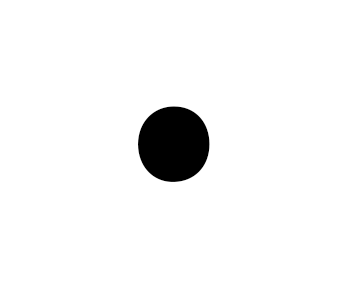
\includegraphics{fig1.png}}
% \caption{Example of a figure caption.}
% \label{fig}
% \end{figure}